\documentclass[tikz]{standalone}
\usetikzlibrary{backgrounds}	% Frame around tikzpicture
\usetikzlibrary{shapes.symbols}	% Wavy rectangle
% \usepackage[none]{hyphenat}		% Prevent hyphenation

\tikzset{
	bed/.pic = {
		\draw [line width=0.3mm] (0,0) rectangle (3,6);
		\draw [] (0,0) rectangle (3,4.5);
	}
}
\tikzset{
	head/.pic = {
		\draw [fill=white] (1.5,5.1) circle (6mm);
		\draw [fill=black] (1.29,5.28) circle (0.6mm);
		\draw [fill=black] (1.71,5.28) circle (0.6mm);
		\draw [black] (1.5,5.25) -- (1.59,4.98) -- (1.47,4.98);
	}
}

\tikzstyle{mytape} = [tape, fill=red, minimum width=3cm, anchor=south west, tape bend bottom=none, tape bend height=2mm, yshift=-1mm]
\tikzstyle{pid} = [fill=white, draw=black, anchor=south, yshift=1mm]

\begin{document}
	
	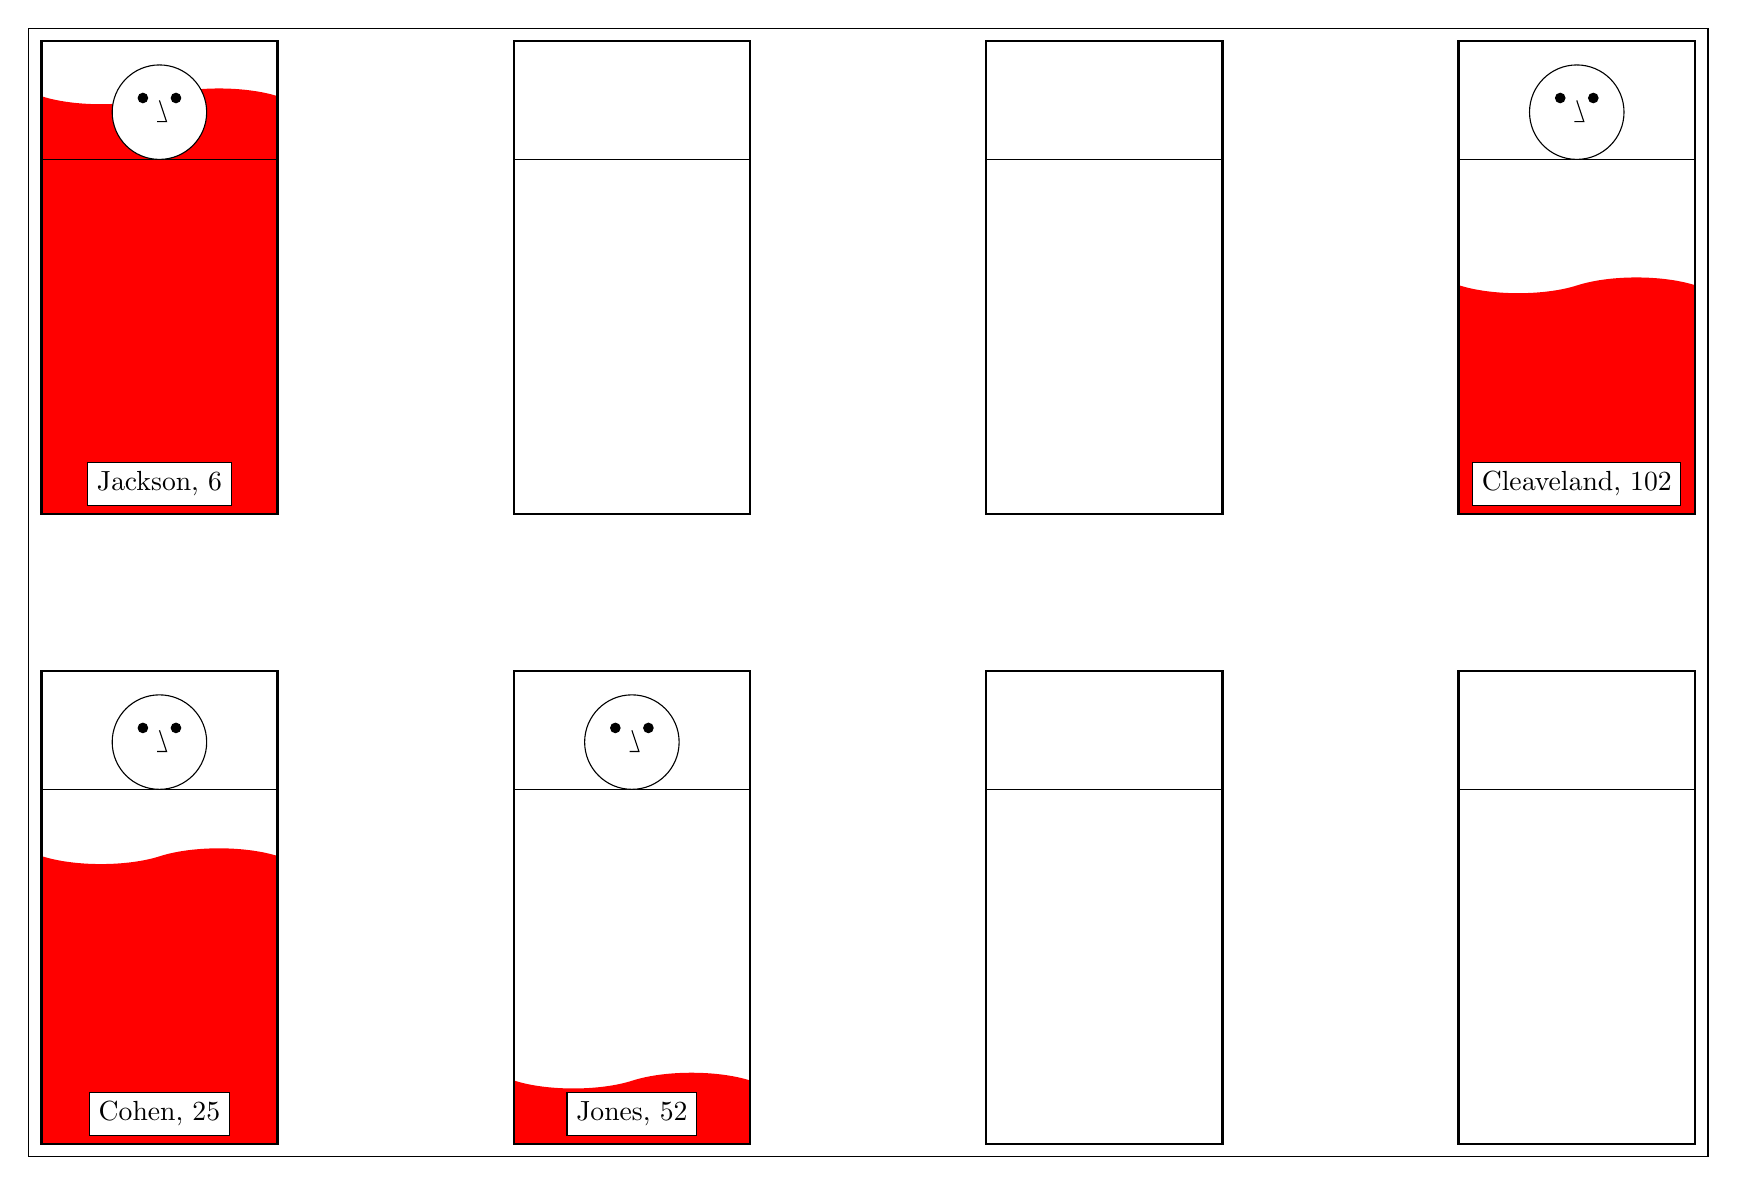
\begin{tikzpicture}[framed, node distance=15mm]

		\node [mytape, minimum height=3.75cm] at (0,0) {};
		\path (0,0) pic{bed};
		\path (0,0) pic{head};
		\node [pid] at (1.5,0) {Cohen, 25};

		\node [mytape, minimum height=0.9cm] at (6,0) {};
		\path (6,0) pic{bed};
		\path (6,0) pic{head};
		\node [pid] at (7.5,0) {Jones, 52};

		\path (12,0) pic{bed};

		\path (18,0) pic{bed};


		\node [mytape, minimum height=5.4cm] at (0,8) {};
		\path (0,8) pic{bed};
		\path (0,8) pic{head};
		\node [pid] at (1.5,8) {Jackson, 6};

		\path (6,8) pic{bed};

		\path (12,8) pic{bed};

		\node [mytape, minimum height=3cm] at (18,8) {};
		\path (18,8) pic{bed};
		\path (18,8) pic{head};
		\node [pid] at (19.5,8) {Cleaveland, 102};

	\end{tikzpicture}
		
\end{document}